% Phase 4 EDA evidence; TRAIN-only descriptive, TEST counts for audit only.
\chapter{Bộ dữ liệu UNSW-NB15 và phân tích dữ liệu}
\label{chap:dataset-eda}

\section{Nguồn dữ liệu và quy mô bản ghi}
UNSW-NB15 là bộ dữ liệu mô tả lưu lượng mạng dùng trong nghiên cứu phát hiện xâm nhập, được giới thiệu trong công bố của Moustafa và Slay \cite{moustafa2015unsw}. Đề tài sử dụng chính xác hai file phân chia chính thức: 175\,341 dòng TRAIN và 82\,332 dòng TEST. Mục tiêu thực nghiệm được kiểm chứng là phân loại \emph{Normal/Attack}; tên các nhóm tấn công không được sử dụng làm predictor trong mô hình binary.

\begin{table}[htbp]\centering
\caption{Phân bố hai lớp của các tập UNSW-NB15 chính thức.}
\label{tab:dist-normal-attack}
\begin{tabular}{lrrrr}\toprule
Tập & Normal & Attack & Tổng & Attack (\%)\\\midrule
TRAIN & 56\,000 & 119\,341 & 175\,341 & 68.06\\
TEST & 37\,000 & 45\,332 & 82\,332 & 55.06\\\bottomrule
\end{tabular}
\end{table}
Sự khác biệt tỷ lệ Attack giữa TRAIN (68,06\%) và TEST (55,06\%) là một quan sát thực tế của dữ liệu chính thức, không phải tỷ lệ do nghiên cứu tự cân bằng lại. Điều này cho thấy tổng Accuracy và Weighted-F1 có thể chịu ảnh hưởng của cách phân bố lớp; đọc Macro-F1, MCC và chỉ số riêng từng lớp sẽ rõ ràng hơn khi so sánh các pipeline.

\begin{figure}[htbp]
\centering
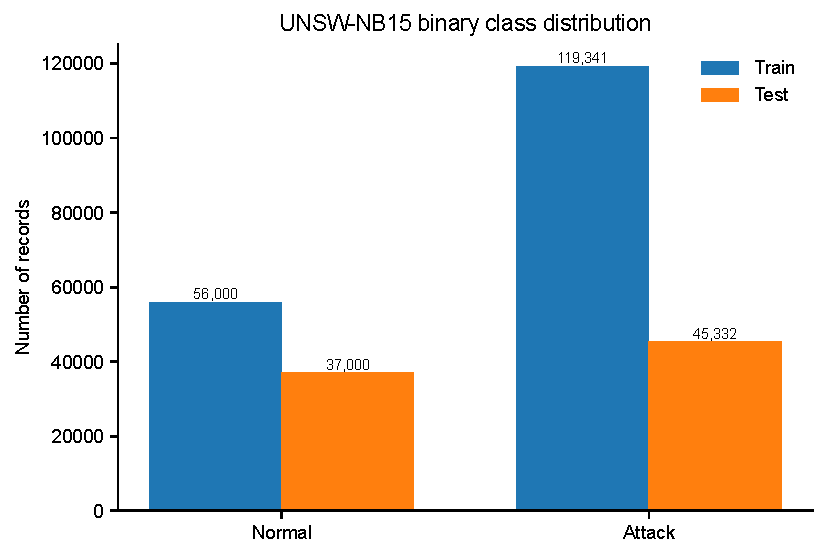
\includegraphics[width=0.86\textwidth]{../results/eda/unsw_nb15/figures/fig01_binary_class_distribution.pdf}
\caption{Phân bố nhãn Normal/Attack trong official TRAIN và TEST, tái sử dụng hình EDA đã lưu ở Phase 4.}
\label{fig:eda-binary}
\end{figure}

\section{Các nhóm tấn công và mức độ chênh lệch}
Ngoài lớp Normal, trường \texttt{attack\_cat} chứa các họ tấn công như Analysis, Backdoor, DoS, Exploits, Fuzzers, Generic, Reconnaissance, Shellcode và Worms. Tại official TEST, Generic chiếm 18\,871 dòng, Exploits 11\,132 dòng và Fuzzers 6\,062 dòng, trong khi Worms chỉ có 44 dòng. Quy mô hỗ trợ không đồng đều có thể làm độ chính xác theo từng nhóm biến động mạnh; một số đếm FN cần được đọc cùng mẫu số của chính nhóm Attack tương ứng.

\begin{figure}[htbp]
\centering
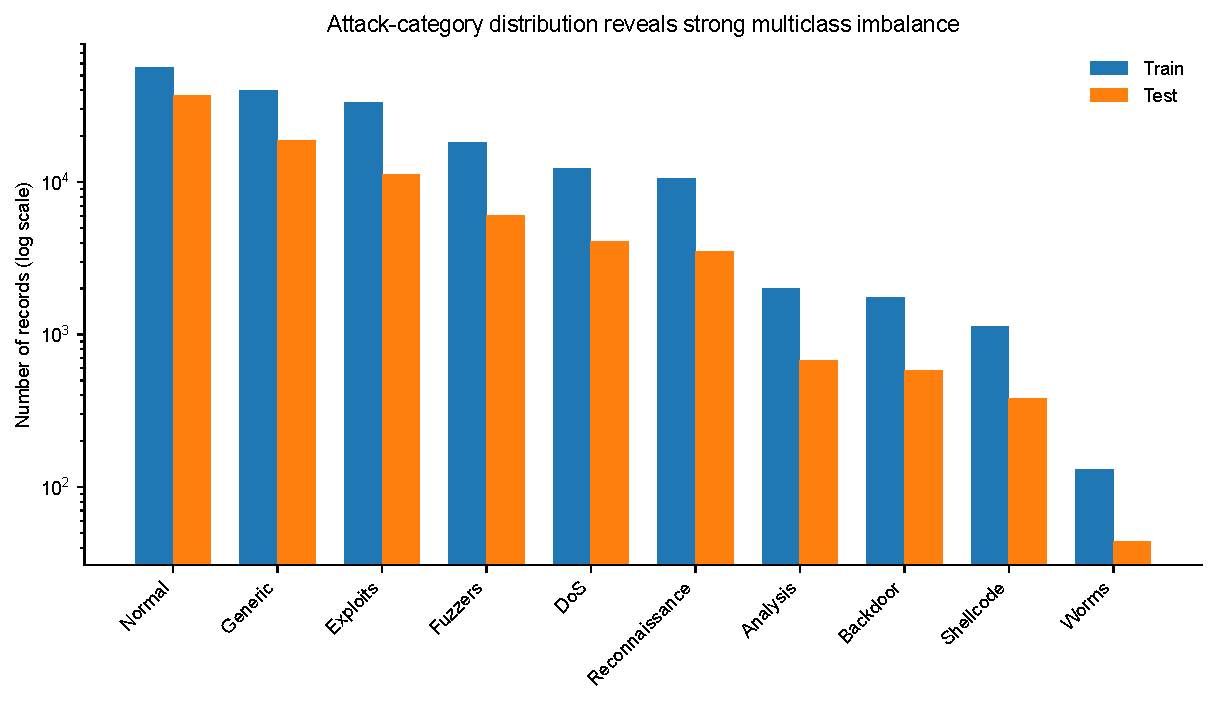
\includegraphics[width=0.94\textwidth]{../results/eda/unsw_nb15/figures/fig02_attack_category_distribution.pdf}
\caption{Số lượng bản ghi theo \texttt{attack\_cat} của hai tập. Trong nghiên cứu hiện tại, đây là phân tích nhãn thật chứ không phải kết quả một mô hình multiclass.}
\label{fig:eda-attackcats}
\end{figure}

Nhóm Attack ít mẫu không thể được coi là đã phát hiện tốt chỉ vì Accuracy nhị phân tổng thể cao. Một lớp hiếm có thể chỉ góp ít FN vào tổng nhưng lại có FNR cao trong chính lớp đó. Bởi vậy bước Error Analysis trong báo cáo phân nhóm các Attack thật, đồng thời tránh biến các khác biệt nhỏ thành khẳng định về toàn bộ dạng tấn công trong tự nhiên.

\section{Khảo sát thống kê các đặc trưng}
EDA của TRAIN đã kiểm tra 39 biến số. Các tiêu chí thống kê dùng để khám phá không đồng nghĩa phép thử nhân quả. Chẳng hạn, standardized mean difference (SMD) giữa Normal và Attack lớn cho thấy trung bình hai nhóm có khác biệt tương đối theo độ phân tán, nhưng không có nghĩa một feature đơn lẻ là dấu hiệu tấn công đáng tin cậy trong mọi tổ hợp.

Các giá trị SMD lớn về độ lớn trong bảng EDA gồm \texttt{sttl} (1,9430), \texttt{ct\_state\_ttl} (1,3973), \texttt{ct\_dst\_sport\_ltm} (0,9340), \texttt{rate} (0,8692), \texttt{ct\_src\_dport\_ltm} (0,7853), cùng các biến có SMD âm như \texttt{swin} (-0,7636) và \texttt{dload} (-0,7346). Dấu và độ lớn của SMD phản ánh cách định nghĩa hai nhóm trong tập TRAIN; nó không thiết lập hướng tác động của feature lên xác suất bị tấn công.

\begin{figure}[htbp]
\centering
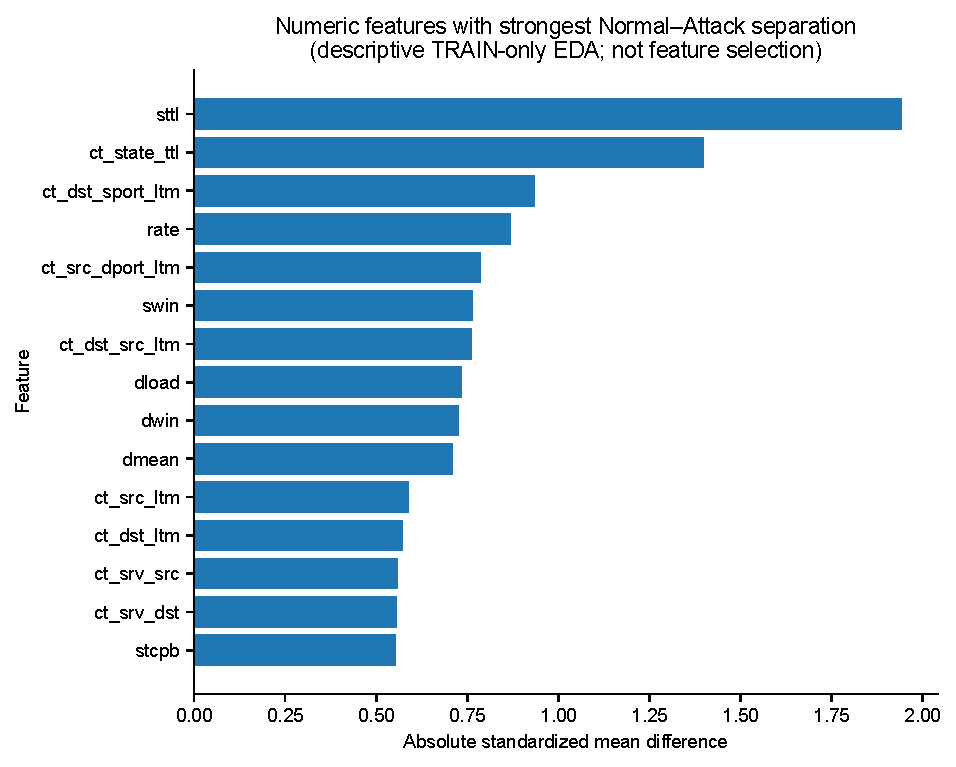
\includegraphics[width=0.96\textwidth]{../results/eda/unsw_nb15/figures/fig03_numeric_class_separation.pdf}
\caption{Khảo sát mức tách biệt Normal/Attack ở một số feature số trên TRAIN (Phase 4). Không dùng biểu đồ này để suy ra quan hệ nhân quả.}
\label{fig:eda-separation}
\end{figure}

\section{Tương quan giữa các đặc trưng}
Trong EDA TRAIN, có 59 cặp feature số đạt $|\rho_{\mathrm{Spearman}}|\geq0,9$. Ví dụ, cặp \texttt{is\_ftp\_login} và \texttt{ct\_ftp\_cmd} có $\rho=1,0000$; \texttt{trans\_depth} và \texttt{ct\_flw\_http\_mthd} có $\rho\approx0,9996$; \texttt{tcprtt} và \texttt{synack} có $\rho\approx0,9968$. Các cặp liên hệ mạnh có thể chứa thông tin trùng lắp trong tập mẫu, nhưng một hệ số tương quan đơn lẻ không cho biết mô hình cây sẽ phụ thuộc vào cặp đó tới mức nào.

\begin{figure}[htbp]
\centering
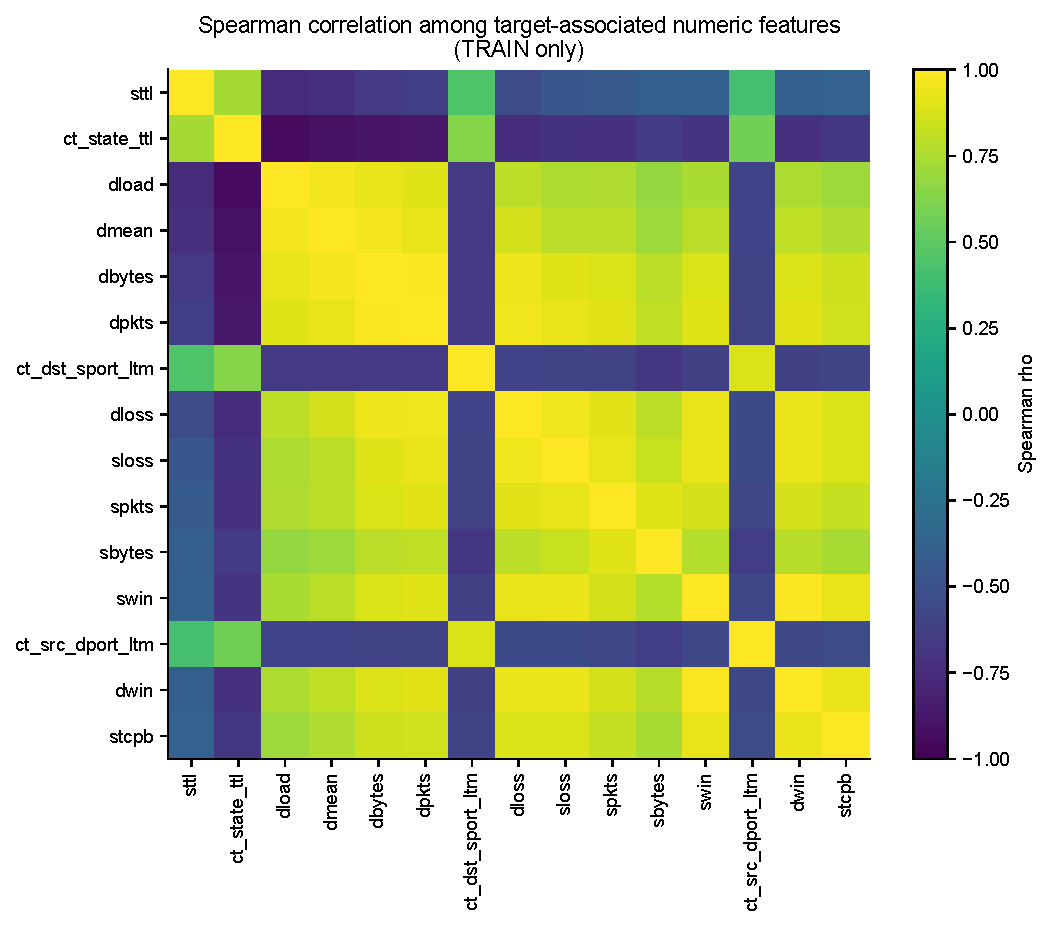
\includegraphics[width=0.96\textwidth]{../results/eda/unsw_nb15/figures/fig04_numeric_correlation_heatmap.pdf}
\caption{Ma trận tương quan các feature số từ Phase 4. Mối tương quan mạnh không tự chứng minh hai biến là tương đương về cơ chế hay có thể loại bỏ không làm mất thông tin.}
\label{fig:eda-correlation}
\end{figure}

Trong bài toán Feature Selection, danh sách cặp tương quan có thể là một trong các nguồn bằng chứng để đề xuất feature candidates, nhưng lựa chọn chính thức còn cần kết hợp kết quả từ filter, embedded và wrapper. Điều quan trọng là giữ phần EDA mô tả tách khỏi quyết định lựa chọn trên validation, không lặng lẽ dùng thông tin từ official TEST để xếp hạng feature.

\section{Kiểm toán overlap và các view đánh giá}
Quy trình audit kiểm tra vector của 42 feature đã sử dụng cho phân loại nhị phân. Có 8\,541 dòng official TEST trùng vector với ít nhất một dòng official TRAIN; phần còn lại gồm 73\,791 dòng được đặt tên \emph{novel-vector view}. Số 8\,541 là \emph{số dòng TEST}, không nhất thiết là số vector riêng biệt hay số session bị giao cắt. Các lớp có thể có giá trị feature giống nhau vì cách lượng hóa và tiền xử lý; vì vậy không được tuyên bố mọi trường hợp trùng vector đều là leakage cùng phiên.

\begin{table}[htbp]\centering
\caption{Hai góc nhìn đánh giá cùng thuộc official TEST đã lưu.}
\label{tab:views-test}
\begin{tabular}{p{0.38\linewidth}r p{0.39\linewidth}}\toprule
View & Số dòng & Diễn giải hợp lệ\\\midrule
Official TEST & 82\,332 & Tập holdout chính thức, dùng cho bảng hiệu năng cuối\\
Novel-vector subset & 73\,791 & TEST sau khi bỏ dòng có vector 42 feature trùng với ít nhất một TRAIN vector\\
Overlap rows & 8\,541 & TEST có vector feature trùng; không tự đồng nhất với cùng session\\\bottomrule
\end{tabular}
\end{table}

Novel-vector view chỉ là một phép phân tích độ nhạy trong cùng bộ dữ liệu, không bảo đảm độc lập theo thời gian hoặc nguồn traffic. Do đó báo cáo trình bày riêng metric official và metric novel-vector, không thay official holdout bằng phần TEST được chọn sau khi quan sát kết quả. Một nghiên cứu đánh giá khả năng khái quát tốt hơn cần một benchmark ngoài hoặc group/temporal split được thiết kế trước, với định nghĩa đơn vị độc lập và quy trình pre-processing nhất quán.

\section{Kết luận về đặc trưng của benchmark}
UNSW-NB15 hỗ trợ một case study IDS nhị phân có quy mô vừa đủ cho đối chiếu nhiều pipeline và có nhãn Attack để phân tích sai số. Tuy nhiên, các chênh lệch lớp, tương quan feature mạnh, sự tồn tại của vector trùng và khả năng phụ thuộc giữa các dòng flow giới hạn phạm vi khái quát. Vì thế hiệu năng trên chính benchmark này được diễn giải dưới các điều kiện của phép đo, không tự chuyển thành khả năng phát hiện xâm nhập trên mạng triển khai thực tế.
